\documentclass[12pt]{article}
\usepackage[utf8]{inputenc}
\usepackage{listings}
\usepackage{amsmath}
\usepackage{float}
\usepackage{graphicx}
\usepackage{subcaption}

\usepackage[
  a4paper,
  left=20mm,
  right=20mm,
  top=20mm,
  bottom=20mm
]{geometry}

\title{Primo report}
\author{Giacomo Longo e Roberta Tassara}
\date{14 Novembre 2019}

\begin{document}
% Titolo
\begin{titlepage}
\maketitle
\end{titlepage}

\section{Analisi di regressione}
\subsection{Introduzione}
Il primo caso che analizzeremo riguarda la realizzazione di una stima mediante un approssimatore universale
$$
  h(x) = \sum_{i=0}^{p} c_i x^i
$$
Tale approssimatore costruisce funzioni del tipo
$$
  h(x) = c_0
$$
$$
  h(x) = c_1 x + c_0
$$
$$
  h(x) = c_2 x^2 + c_1 x + c_o
$$
La funzione ricercata deve minimizzare l'errore empirico
$$
  \underset{\underline{c}}{\min} \{ \frac{1}{n} \sum_{i=1}^{n} (y_i - h(x_i))^2 \}
  \qquad
  \underline{c} = \{ c_0, ..., c_p \}
$$
che rappresenta la somma delle distanze tra i dati osservati ($y_i$) e quelli della curva ottima ($h(x_i)$). \\
Scrivendo la funzione in forma matriciale,
derivandola rispetto a c
e ponendo il tutto $=0$ si ottiene
$$
  \underline{c} = (X^T X)^+ X \underline{y}
$$
che corrisponde al minimo globale

\subsection{Analisi al variare di p con $y=1-x^2$}

\subsubsection{Parametri di simulazione}
Dimensione dell'asse delle x: $10000$ punti \\
Intervallo dell'asse delle x: $0 \leq x \leq 1$ \\
Punti campione: $10$ \\
Intensitá di rumore: $10\%$

\subsubsection{$p>n-1$}
L'analisi é stata omessa in quanto non rilevante: per tracciare $n$ punti é sufficiente un polinomio di grado $n-1$

\subsubsection{$p=n-1$}
Se $p=n-1$ la funzione estimante(in verde) attraversa perfettamente tutti i punti campionati(in rosso),
tuttavia non rappresenta una buona approssimazione della funzione originale (in blu). \\
Infatti l'errore medio individuato é particolarmente alto. \\
Tale risultato, anche in prossimitá dei campioni con valori molto simili alla funzione reale,
la funzione stimata si comporta in modo molto differente con vistose oscillazioni dovute ai termini di grado elevato.

\begin{figure}[H]
  \centering
  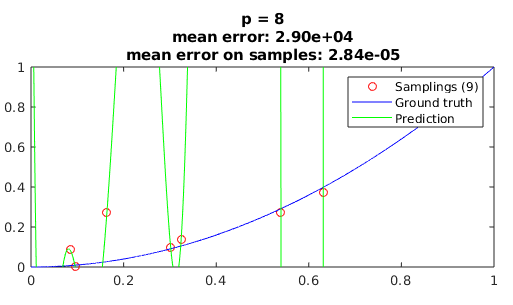
\includegraphics[width=0.75\textwidth]{plots/regression/maximum_p.png}
\end{figure}

\subsubsection{$p<n-1$}

Per bassi valori di p, la funzione risultante é semplice. \\
Tra i vari valori di p, in questa particolare istanza,
il valore che approssima meglio la funzione originale é $p=3$
per il quale si ha il piú basso errore medio. \\
Questo significa che per questa funzione,
l'errore di approssimazione é inferiore a quello di stima. \\
Colpisce anche che il miglior stimatore non coincida con il grado della funzione originaria,
ció é dovuto al rumore. \\

\begin{figure}[H]
  \centering
  \begin{subfigure}{0.45\textwidth}
    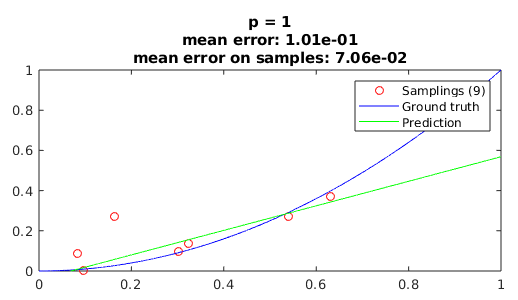
\includegraphics[width=\textwidth]{plots/regression/p_eq_1.png}
  \end{subfigure}
  \begin{subfigure}{0.45\textwidth}
    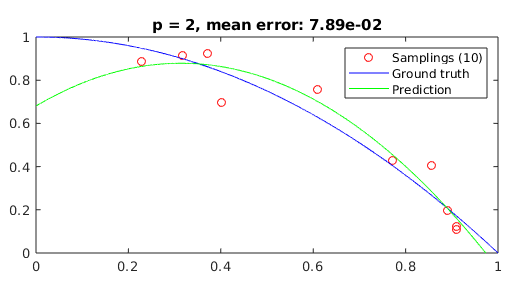
\includegraphics[width=\textwidth]{plots/regression/p_eq_2.png}
  \end{subfigure}
\end{figure}

\begin{figure}[H]
  \centering
  \begin{subfigure}{0.45\textwidth}
    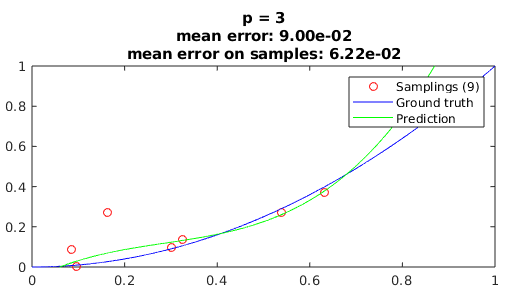
\includegraphics[width=\textwidth]{plots/regression/p_eq_3.png}
  \end{subfigure}
  \begin{subfigure}{0.45\textwidth}
    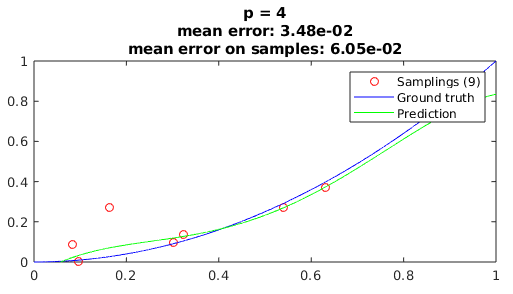
\includegraphics[width=\textwidth]{plots/regression/p_eq_4.png}
  \end{subfigure}
\end{figure}

\begin{figure}[H]
  \centering
  \begin{subfigure}{0.45\textwidth}
    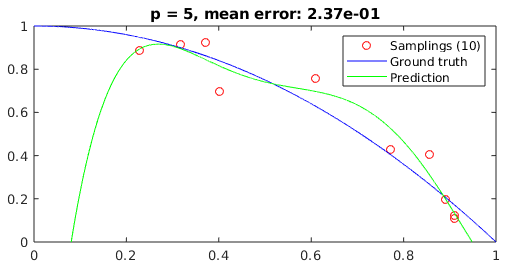
\includegraphics[width=\textwidth]{plots/regression/p_eq_5.png}
  \end{subfigure}
  \begin{subfigure}{0.45\textwidth}
    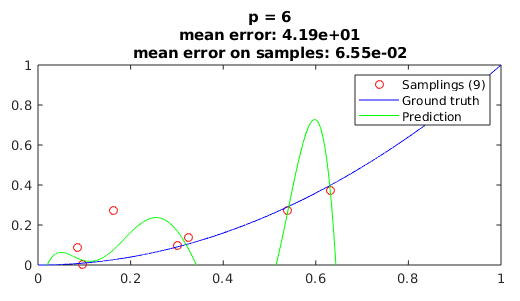
\includegraphics[width=\textwidth]{plots/regression/p_eq_6.png}
  \end{subfigure}
\end{figure}

\begin{figure}[H]
  \centering
  \begin{subfigure}{0.45\textwidth}
    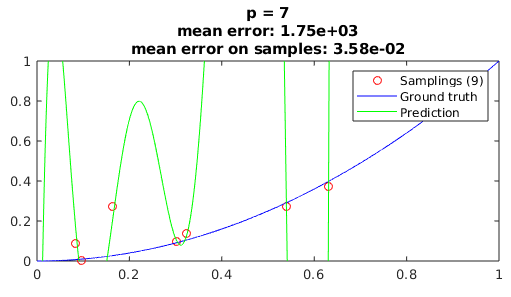
\includegraphics[width=\textwidth]{plots/regression/p_eq_7.png}
  \end{subfigure}
  \begin{subfigure}{0.45\textwidth}
    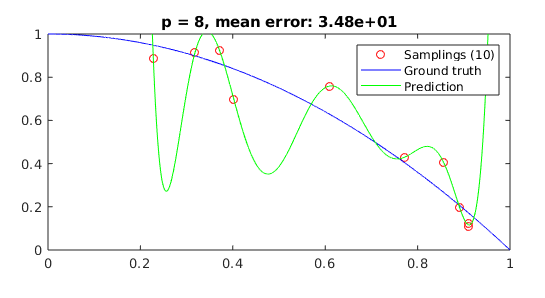
\includegraphics[width=\textwidth]{plots/regression/p_eq_8.png}
  \end{subfigure}
\end{figure}

\newpage
\subsection{Codice}
\lstinputlisting[basicstyle=\tiny ,language=MATLAB]{regressione.m}

\end{document}
